% Add theorem environments
\newtheorem{theorem}{Theorem}
\newtheorem{definition}{Definition}
\section{Learning Goals}

By the end of this chapter, you will:

\begin{itemize}
    \item \textbf{Know what is meant by binary linear classification} and understand its fundamental concepts
    \item \textbf{Understand why an explicit threshold for a classifier is redundant} and how bias terms can be eliminated using dummy features
    \item \textbf{Be able to specify weights and biases by hand} to represent simple logical functions (AND, OR, NOT)
    \item \textbf{Be familiar with input space and weight space}, including:
    \begin{itemize}
        \item Plotting training cases and classification weights in both spaces
        \item Understanding the geometric interpretation of linear classifiers
    \end{itemize}
    \item \textbf{Be aware of the limitations of linear classifiers}, including:
    \begin{itemize}
        \item Understanding convexity and its role in linear separability
        \item Knowing how basis function representations can overcome some limitations
    \end{itemize}
\end{itemize}

\section{Fundas: Mathematical Foundations}

\begin{fundasblock}{Mathematical Foundations}
\subsection{Vector Representation}
\begin{itemize}
    \item \textbf{Input vectors}: Each data point is represented as a $D$-dimensional vector $\bm{x}^{(i)} = [x_1^{(i)}, x_2^{(i)}, \ldots, x_D^{(i)}]$
    \item \textbf{Weight vectors}: Classification parameters represented as $\bm{w} = [w_1, w_2, \ldots, w_D]$
    \item \textbf{Linear combination}: $f(\bm{x}) = \bm{w}^T\bm{x} + b$, where $b$ is the bias term
    \item \textbf{Decision boundary}: The hyperplane where $\bm{w}^T\bm{x} + b = 0$
\end{itemize}

\subsection{Binary Classification Framework}
\begin{itemize}
    \item \textbf{Target values}: $t^{(i)} \in \{0, 1\}$ where $0 =$ negative class, $1 =$ positive class
    \item \textbf{Classification rule}: $\hat{y} = 1$ if $\bm{w}^T\bm{x} + b > \tau$, else $\hat{y} = 0$ (where $\tau$ is threshold)
    \item \textbf{Training set}: $\{(\bm{x}^{(i)}, t^{(i)})\}_{i=1}^N$ where $N$ is the number of examples
\end{itemize}
\end{fundasblock}

\textbf{What is Hyperplane ?} 
\begin{definition}[Hyperplane]
A hyperplane in a $D$-dimensional space is a flat affine subspace of dimension $D-1$. It can be defined by a linear equation of the form:
\begin{equation}
\bm{w}^T \bm{x} + b = 0
\end{equation}
where $\bm{w}$ is a normal vector to the hyperplane, $\bm{x}$ is a point on the hyperplane, and $b$ is the bias term.
\end{definition}
\textbf{Properties of Hyperplanes}:
\begin{itemize}
    \item \textbf{Normal Vector}: The weight vector \(\mathbf{w}\) is perpendicular to the decision boundary
    \item \textbf{Distance from Origin}: \(\frac{|b|}{||\mathbf{w}||_2}\) gives the perpendicular distance from the hyperplane to the origin
    \item \textbf{Classification Rule}:
    \begin{itemize}
        \item Points where \(\mathbf{w}^T \mathbf{x} + b > 0\) are classified as positive halfspcace (class 1)
        \item Points where \(\mathbf{w}^T \mathbf{x} + b < 0\) are classified as negative halfspace (class 0)
        \item Points on the boundary satisfy \(\mathbf{w}^T \mathbf{x} + b = 0\)
    \end{itemize}
\end{itemize}
\begin{figure}
    \centering
    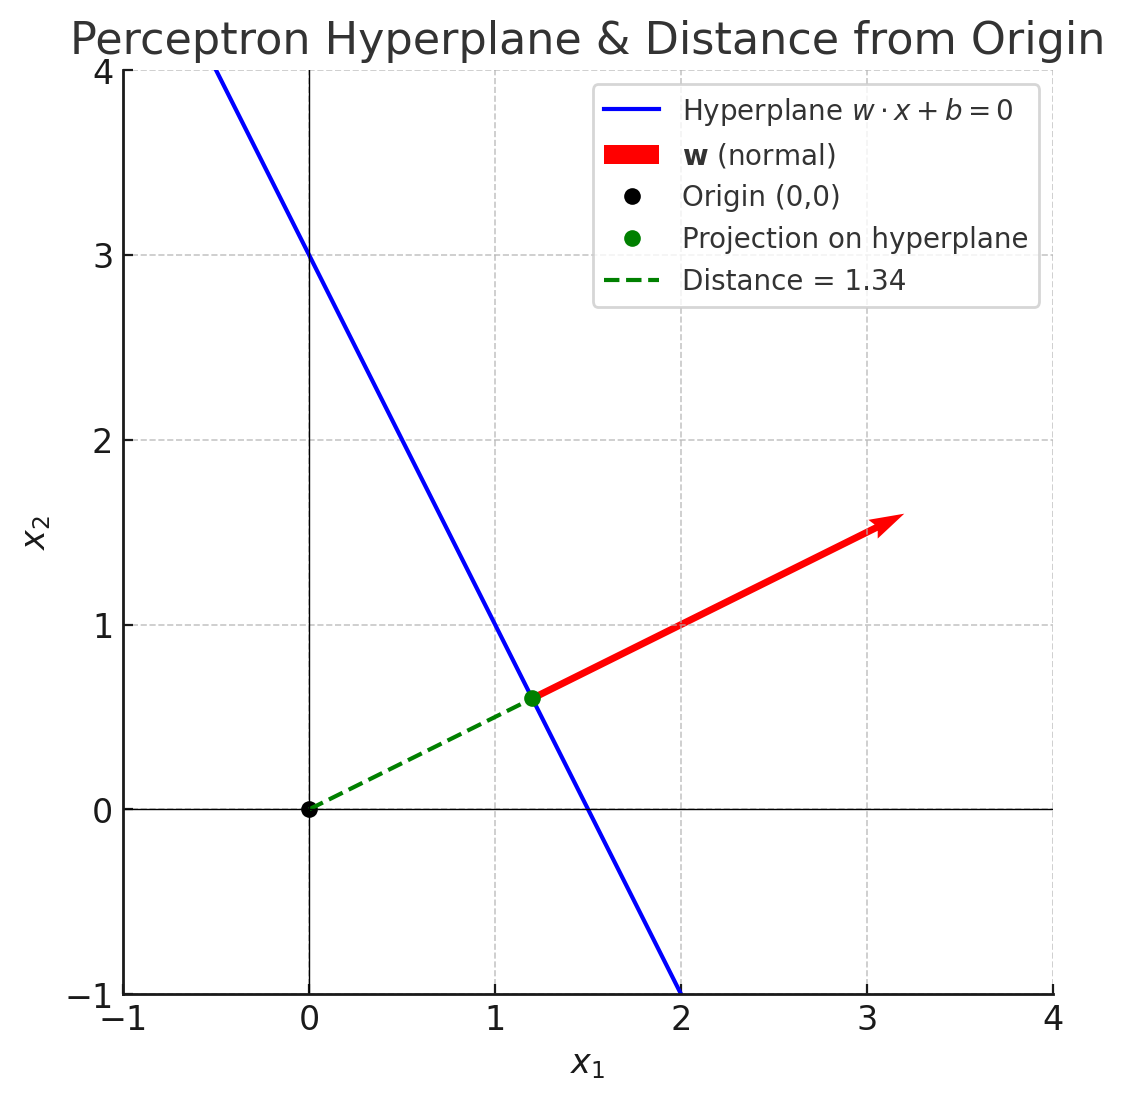
\includegraphics[width=0.6\textwidth]{input_space.png}
    \caption{Hyperplane in 2D input space. The line represents the decision boundary where $\bm{w}^T \bm{x} + b = 0$.}
    \label{fig:input_space} 
\end{figure}

\textbf{Distance of a point from the Hyperplane}

The distance \(d\) of a point \(\mathbf{x}_i\) from the hyperplane defined by \(\mathbf{w}^T \mathbf{x} + b = 0\) is given by the formula:
\[
d = \frac{|\mathbf{w}^T \mathbf{x}_i + b|}{||\mathbf{w}||_2}
\]

Where:  
\begin{itemize}
    \item \(\mathbf{w}^T \mathbf{x}_i + b\) is the signed distance from the hyperplane (positive if on the positive side, negative if on the negative side)
    \item \(||\mathbf{w}||_2\) is the Euclidean norm of the weight vector, which normalizes the distance
    \item The absolute value ensures the distance is non-negative
\end{itemize}



\textbf{Example}: 
\begin{itemize}
    \item If $y_i = +1$ (positive class) and $\mathbf{w}^T \mathbf{x}_i = +2.5$ → product = $+2.5$ $\checkmark$ (correct)
    \item If $y_i = +1$ (positive class) and $\mathbf{w}^T \mathbf{x}_i = -1.2$ → product = $-1.2$ $\times$ (incorrect)
    \item If $y_i = -1$ (negative class) and $\mathbf{w}^T \mathbf{x}_i = -0.8$ → product = $+0.8$ $\checkmark$ (correct)
\end{itemize}


\textbf{What is Linearly Separable?}
\begin{definition}[Linear Separability]
A dataset is said to be linearly separable if there exists a hyperplane that can separate all positive examples from all negative examples without any misclassification.
\end{definition}
\textbf{Implications of Linear Separability}:
\begin{itemize}
    \item If a dataset is linearly separable, a linear classifier can achieve perfect classification
    \item If not, more complex models or feature transformations may be necessary
\end{itemize}   
\textbf{Why Hyperplanes Matter in Linear Classification?}
\begin{itemize}
    \item In binary linear classification, the decision boundary is represented by a hyperplane
    \item The hyperplane separates the input space into two regions corresponding to the two classes
    \item The orientation and position of the hyperplane are determined by the weights $\bm{w}$ and bias $b$
\end{itemize}

\section{Introduction to Binary Classification}

Binary classification represents one of the most fundamental problems in machine learning, where the goal is to predict a binary-valued target from input features. This forms the foundation for understanding more complex classification scenarios.

\subsection{Real-World Applications}

\subsubsection{Medical Diagnosis Systems}
\begin{itemize}
    \item \textbf{Problem}: Predict whether a patient has a specific disease
    \item \textbf{Features}: Symptoms, test results, patient history
    \item \textbf{Target}: Disease present (1) or absent (0)
    \item \textbf{Example}: Diagnosing diabetes from glucose levels, BMI, and family history
\end{itemize}

\subsubsection{Email Spam Detection}
\begin{itemize}
    \item \textbf{Problem}: Classify emails as spam or legitimate
    \item \textbf{Features}: Word frequencies, sender information, email metadata
    \item \textbf{Target}: Spam (1) or not spam (0)
    \item \textbf{Example}: Using keywords like ``free money'' as indicators
\end{itemize}

\subsubsection{Fraud Detection}
\begin{itemize}
    \item \textbf{Problem}: Identify fraudulent transactions
    \item \textbf{Features}: Transaction amount, time, location, merchant type
    \item \textbf{Target}: Fraudulent (1) or legitimate (0)
    \item \textbf{Example}: Detecting unusual spending patterns
\end{itemize}

\section{Binary Linear Classifiers: First Principles}

\subsection{Core Concept}

A binary linear classifier makes decisions by computing a linear function of the input features and comparing the result to a threshold. This approach assumes that the two classes can be separated by a linear decision boundary in the feature space.

\begin{figure}
    \centering
    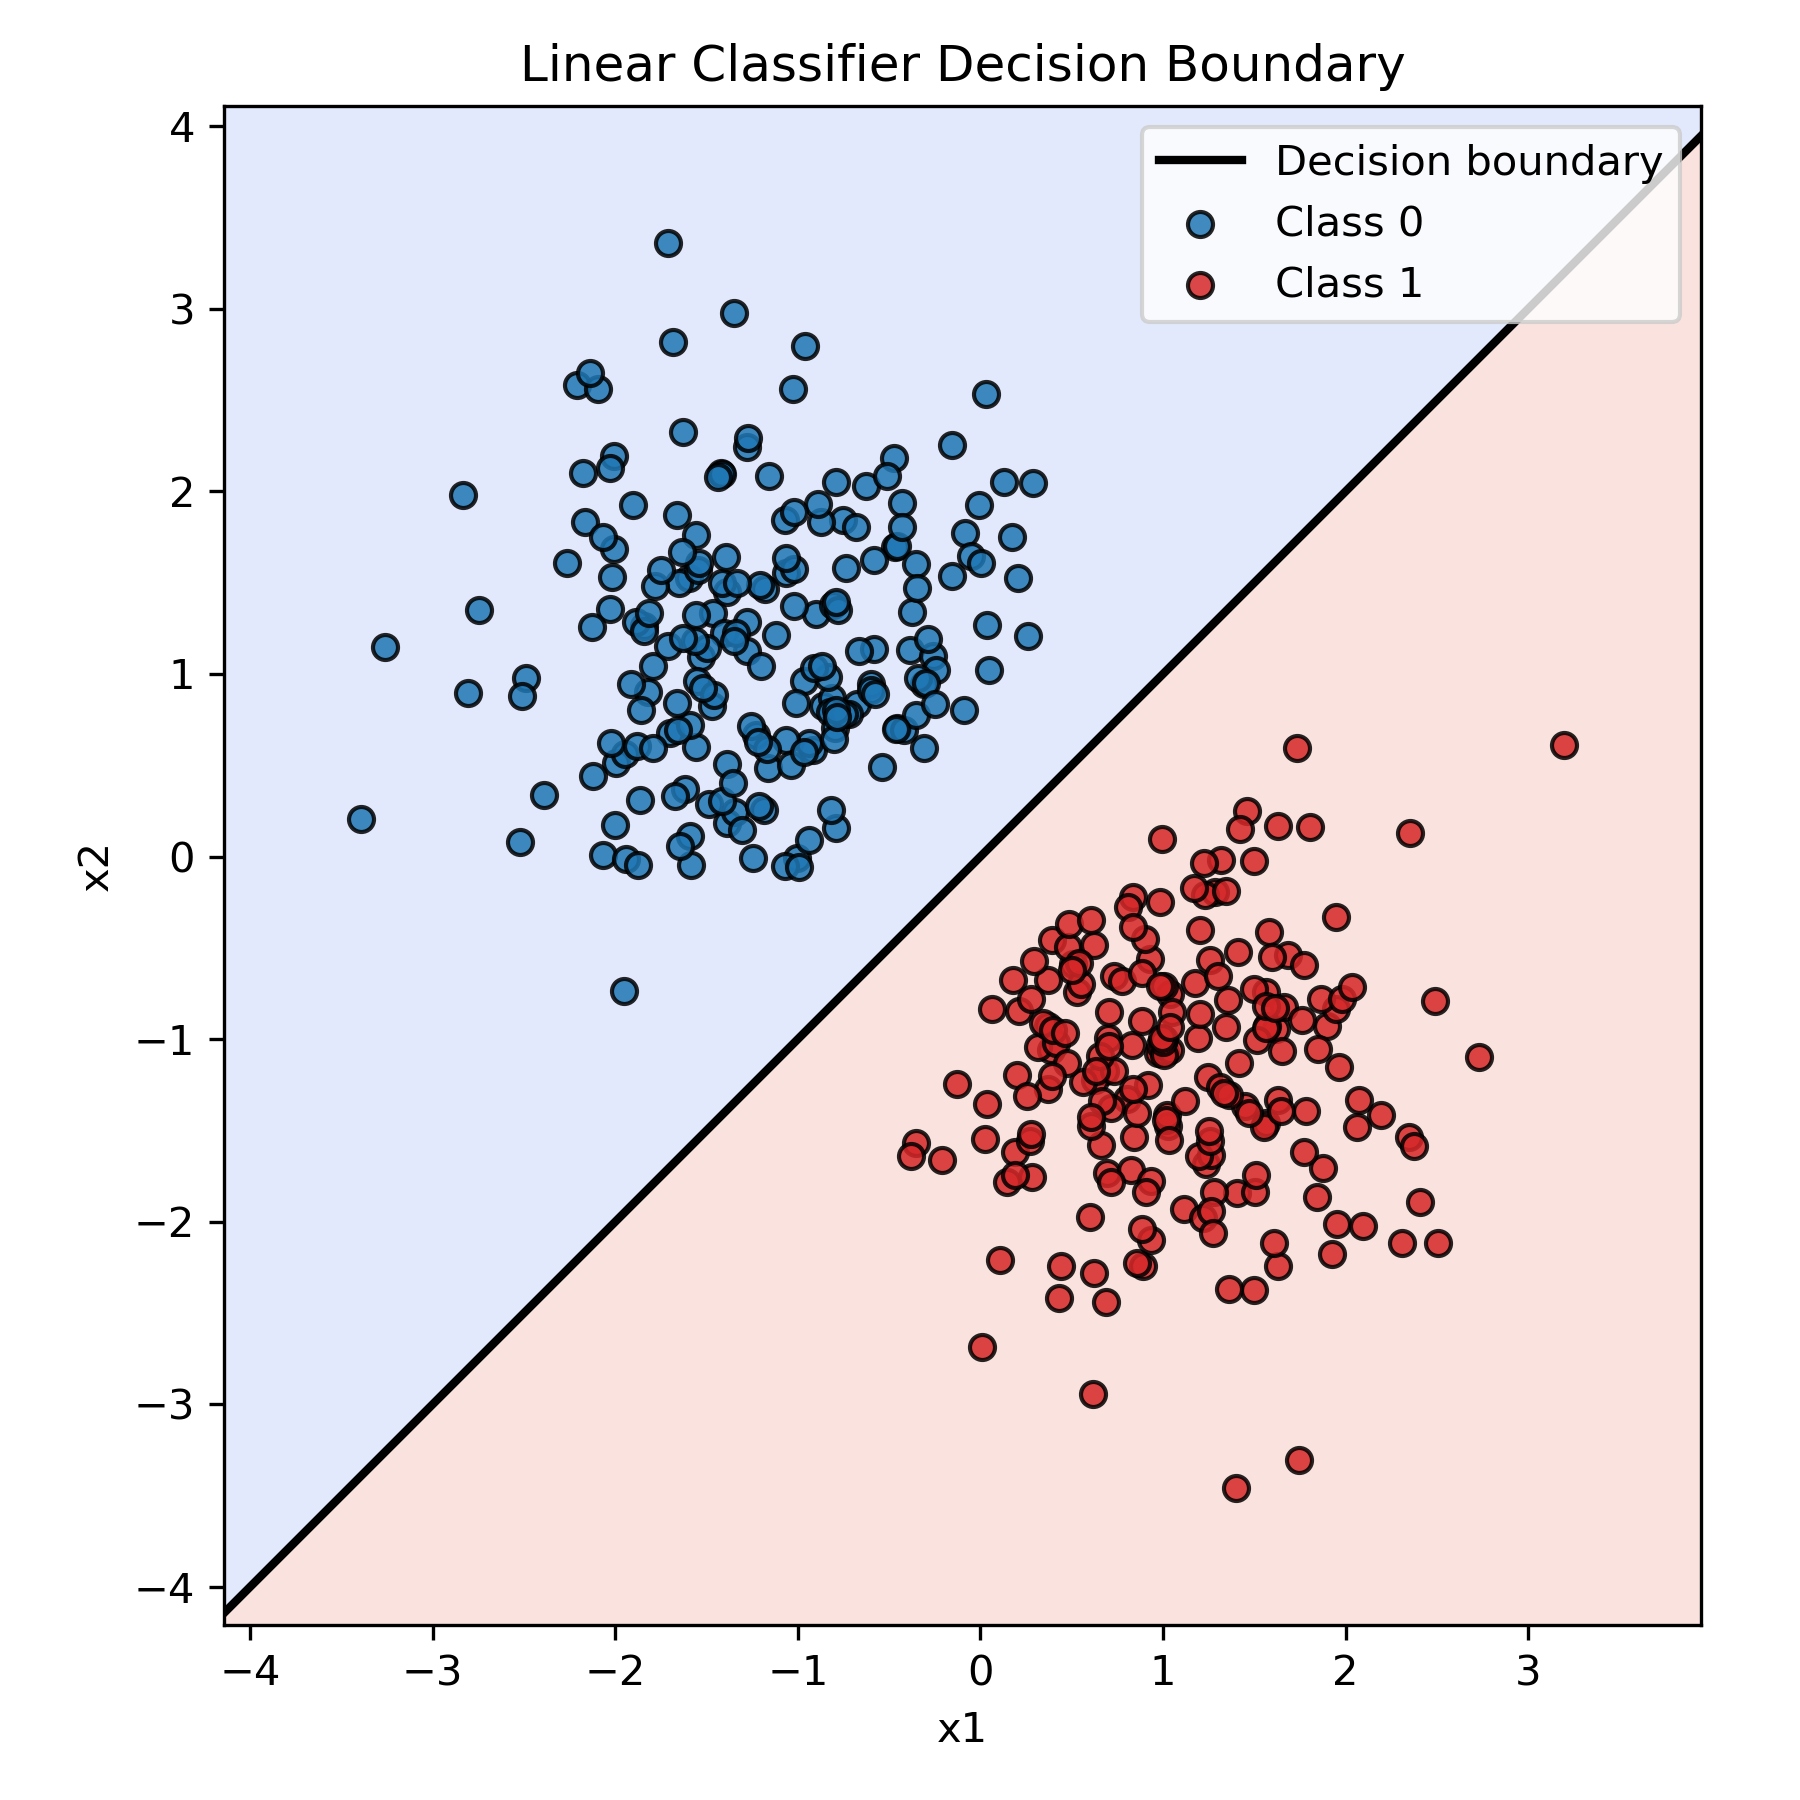
\includegraphics[width=0.6\textwidth]{linear_classifier_decision_boundary.png}
    \caption{A simple binary linear classifier with two features. The decision boundary (line) separates the two classes.}
    \label{fig:linear_classifier}
\end{figure}


\subsection{Mathematical Formulation}

\textbf{Step 1: Linear Combination}
\begin{equation}
z = w_1x_1 + w_2x_2 + \cdots + w_D x_D + b = w^{T}\bm{x} + b
y = \begin{cases}
1 & \text{if } z \geq \tau \\
0 & \text{otherwise}
\end{cases}
\end{equation}


\textbf{Step 2: Threshold Decision}
\begin{equation}
\hat{y} = \begin{cases}
1 & \text{if } z > \tau \\
0 & \text{otherwise}
\end{cases}
\end{equation}

Where:
\begin{itemize}
    \item $w_i$: Weight for feature $i$ (determines importance and direction)
    \item $x_i$: Value of feature $i$
    \item $b$: Bias term (shifts the decision boundary)
    \item $\tau$: Threshold value
\end{itemize}

\subsection{Eliminating Redundancy: The Bias-Threshold Trick}

\textbf{Problem}: Having both bias ($b$) and threshold ($\tau$) is redundant.

\textbf{Step 1}: Absorb threshold into bias term:
\begin{itemize}
    \item Set new bias: $b' = b - \tau$
    \item Set threshold to zero: $\tau = 0$
    \item Decision rule becomes: $\hat{y} = 1$ if $\bm{w}^T\bm{x} + b' > 0$
\end{itemize}

\textbf{Step 2}: Add dummy feature:
\begin{itemize}
    \item Extend input: $\bm{x} \rightarrow [\bm{x}, 1]$
    \item Extend weights: $\bm{w} \rightarrow [\bm{w}, b']$
    \item Decision rule: $\hat{y} = 1$ if $\bm{w}_{\text{extended}}^T \bm{x}_{\text{extended}} > 0$
\end{itemize}
\begin{block}{Note}
Without loss of generality, we can say $z = \bm{w}^{T}\bm{x}$
\end{block}

\subsection{Some Examples}

\textbf{Example 1}: For NOT gate \\

\textbf{Truth Table}: \\

\begin{tabular}{|c|c|}
\hline
Input & Output \\
\hline
0 & 1 \\
\hline
1 & 0 \\
\hline
\end{tabular}

\begin{itemize}
    \item Each of the traning cases provides a constraint on the weights and biases. 
    \item For example, the first training case $(0,1)$ requires that $z = 0 \cdot w_1 + b \geq 0$, which simplifies to $b \geq 0$. Technically $b$ can be $0$ but it is good practice to avoid the solutions which lies on decision boundary, so let us take tentatively $b=1$.
    \item The second training case $(1,0)$ requires that $z = 1 \cdot w_1  + b < 0$. We can satisfy this inequality by setting $w_1 = -2$.
    \item Thus, we have $w_1 = -2$ and $b = 1$.
\end{itemize}


\textbf{Example 2}: For AND gate \\

\textbf{Truth Table}: \\

\begin{tabular}{|c|c|c|}
\hline
Input 1 & Input 2 & Output \\
\hline
0 & 0 & 0 \\
\hline
0 & 1 & 0 \\
\hline
1 & 0 & 0 \\
\hline
1 & 1 & 1 \\
\hline
\end{tabular}   

\begin{align*}
\text{Case }(0,0): & \quad b < 0 \quad  \\
\text{Case }(0,1): & \quad w_2 + b < 0 \\
\text{Case }(1,0): & \quad w_1 + b < 0 \quad \\
\text{Case }(1,1): & \quad w_1 + w_2 + b \geq 0 
\end{align*}    

Normally finding the weights and biases are a bit of trial and error. But let us try to solve it systematically.
\begin{itemize}
    \item From the first case, we can set $b < 0$ 
    \item From the fourth, it seems that $w_1$ and $w_2$ must be positive.
    \item Since the problem is symmetric in $w_1$ and $w_2$, let us set $w_1 = w_2 = w > 0$.
    \item Now, the second and third cases become $w + b < 0$
    \item The fourth case becomes $2w + b \geq 0$
    \item Let us set $b = -1$ (satisfies the first case)
    \item Then, $w - 1 < 0$ implies $w < 1$ and $2w - 1 \geq 0$ implies $w \geq 0.5$
    \item We can satisfy both by setting $w = 0.5$
    \item Thus, we have $w_1 = 0.5$, $w_2 = 0.5$ and $b = -1$
\end{itemize}



\section{Geometric Interpretation}


\subsection{Data Space}
\begin{itemize}
    \item \textbf{Data Space (Input Space)}: The first space to be familiar with is data space, or input space. Each point in this space corresponds to a possible input vector.
        \item \textbf{Representation of Examples}: It's customary to represent positive and negative examples with the symbols "+" and "-", respectively.
        
        \item \textbf{Division of Space}: Once we've chosen the weights $\bm{w}$ and bias $b$, we can divide the data space into a region where the points are classified as positive (the positive region), and a region where the points are classified as negative (the negative region).
    
        \item \textbf{Decision Boundary}: The boundary between these regions, i.e., the set where $\bm{w}^T \bm{x} + b = 0$, is called the decision boundary. Think back to your linear algebra class, and recall that the set determined by this equation is a hyperplane.
        
        \item \textbf{Half-Space}: The set of points on one side of the hyperplane is called a half-space.
\end{itemize}


\textbf{Decision Boundary}: The hyperplane $\bm{w}^T\bm{x} + b = 0$ divides the input space into two regions:
\begin{itemize}
    \item \textbf{Positive region}: $\bm{w}^T\bm{x} + b > 0$ (predicted class 1)
    \item \textbf{Negative region}: $\bm{w}^T\bm{x} + b < 0$ (predicted class 0)
\end{itemize}

\subsection{Weight Space}
\begin{itemize}
    \item Each point in weight space corresponds to a weight vector $\bm{w}$ . Here we will not consider the bias terms explicitly, since we can always absorb them into the weights by adding a dummy feature to the input vectors.
    \item Each training example imposes a constraint on the weights. For example, if we have a positive example $\bm{x}^{(i)}$, then we must have $\bm{w}^T\bm{x}^{(i)}  > 0$ in order to classify it correctly. The set of points in weight space that satisfy this inequality is a half-space.
    \item Similarly, a negative example $\bm{x}^{(j)}$ imposes the constraint $\bm{w}^T\bm{x}^{(j)} < 0$, which also defines a half-space in weight space.
    \item Each training example thus carves out a half-space in weight space.
    \item The intersection of all these half-spaces defines the region of weight vectors that correctly classify all training examples which is called the \textbf{feasible region}.
\end{itemize}


\subsection{Illustrating Input Space and Weight Space with the NOT Function}
The input matrix is given by after applying the bias trick(that is $x_{0} = 1$):
\begin{equation}
X = \begin{bmatrix}
1 & 0 \\
1 & 1
\end{bmatrix}
\end{equation}

\begin{figure}
    \centering
    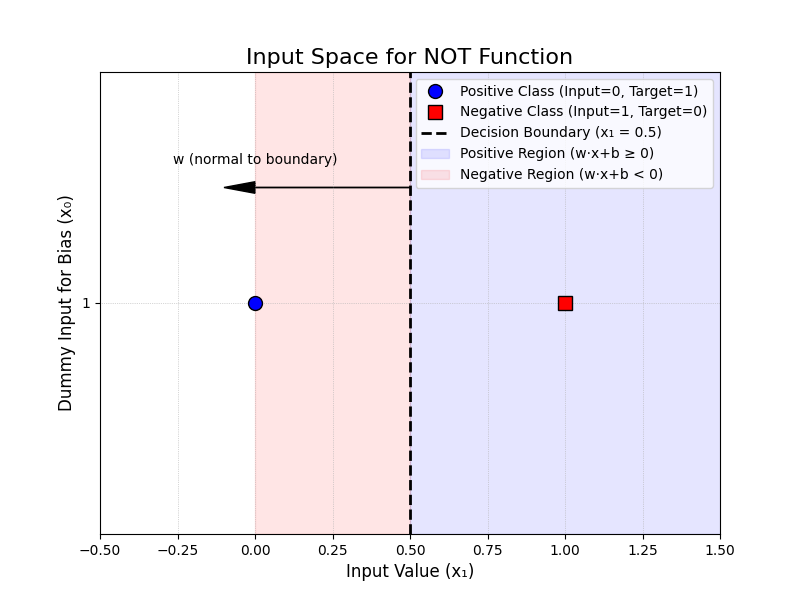
\includegraphics[width=0.6\textwidth]{not_input_space.png}
    \caption{Input space for the NOT function using the bias trick. The decision boundary is $x_1 = -\frac{b}{w_1}$.}
    \label{fig:not_input_space}     
\end{figure}

\subsubsection{Weight Space Visualization}

The bias trick will give us \([w_{0}, w_{1}]\) as the weight vector. The constraints from the training examples are:
\begin{align}
\text{For }(0,1): & \quad w_{0} > 0 \\
\text{For }(1,0): & \quad w_{1} + w_{0} < 0
\end{align} 
\textbf{Plotting the Constraints}:
\begin{itemize}
    \item The first constraint \(w_{0} > 0\) corresponds to the half-space above the line \(w_{0} = 0\).
    \item The second constraint \(w_{1} + w_{0} < 0\) can be rearranged to \(w_{0} < -w_{1}\), which corresponds to the half-space below the line \(w_{0} = -w_{1}\).
\end{itemize}       
The feasible region is where both constraints are satisfied.

\begin{figure}[htbp]
    \centering
    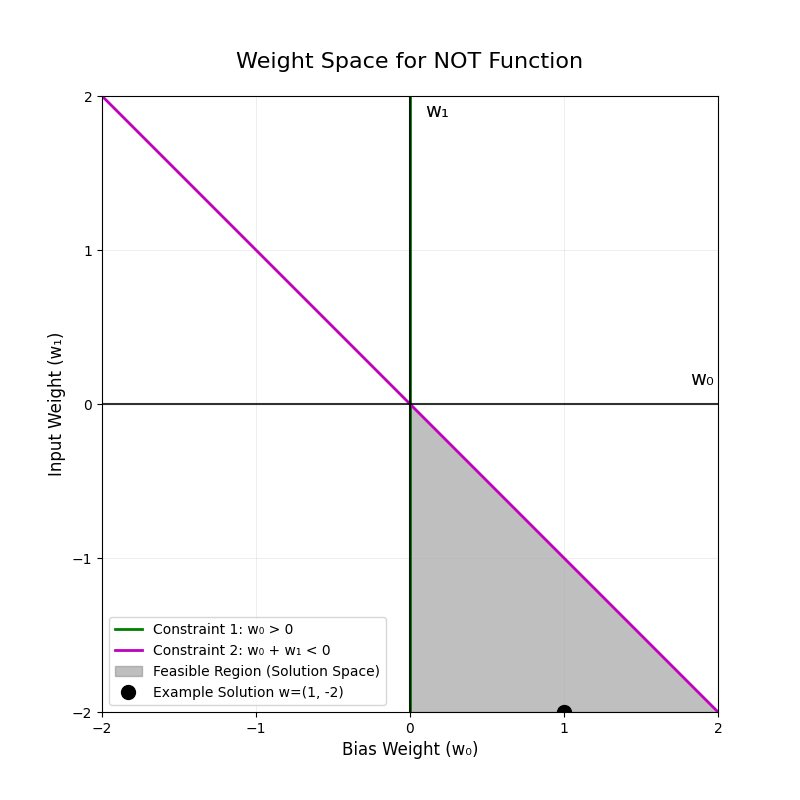
\includegraphics[width=0.6\textwidth]{not_weight_space.png}
    \caption{Weight space for the NOT function using the bias trick. The feasible region is $b > 0$ and $w_1 + b < 0$.}
    \label{fig:not_weight_space}
\end{figure}

\subsection{Illustrating Input Space and Weight Space with the AND Function}
The input matrix is given by after applying the bias trick(that is $x_{0} = 1$):
\begin{equation}
X = \begin{bmatrix}
1 & 0 & 0 \\
1 & 0 & 1 \\
1 & 1 & 0 \\
1 & 1 & 1
\end{bmatrix}
\end{equation}      

\begin{figure}
    \centering
    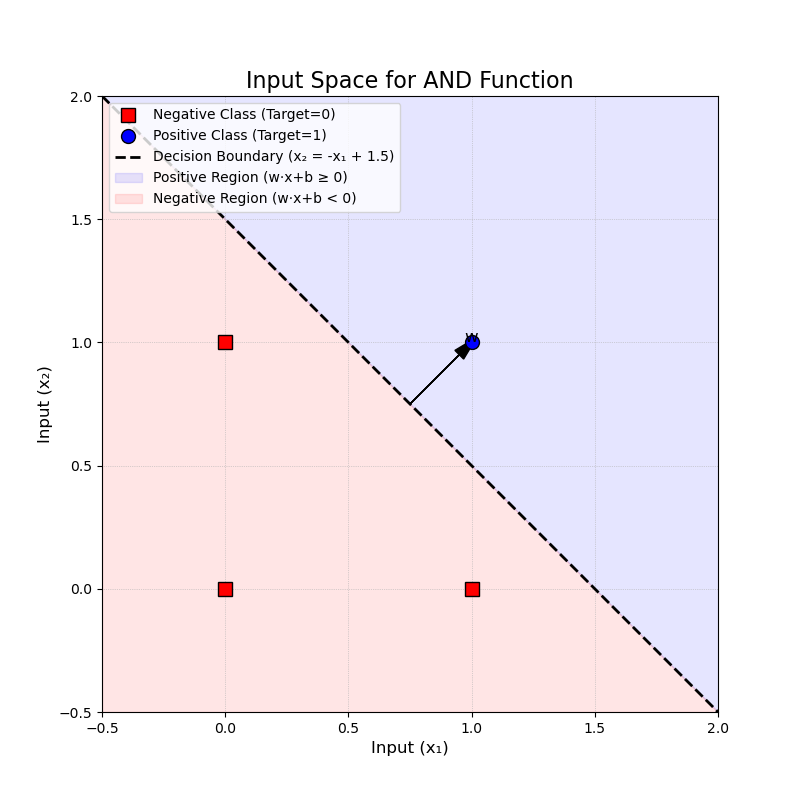
\includegraphics[width=0.6\textwidth]{and_input_space.png}
    \caption{Input space for the AND function using the bias trick. The decision boundary is $x_1 + x_2 = -\frac{b}{w_1}$.}
    \label{fig:and_input_space}    
\end{figure}        
\subsubsection{Weight Space Visualization}  
The bias trick will give us \([w_{0}, w_{1}, w_{2}]\) as the weight vector. The constraints from the training examples are:
\begin{align}
\text{For }(0,0): & \quad w_{0} < 0 \\
\text{For }(0,1): & \quad w_{2} + w_{0} < 0 \\
\text{For }(1,0): & \quad w_{1} + w_{0} < 0 \\
\text{For }(1,1): & \quad w_{1} + w_{2} < 0             
\end{align}
\textbf{Plotting the Constraints}:
\begin{itemize}
    \item The first constraint \(w_{0} < 0\) corresponds to the half-space below the line \(w_{0} = -0.3\).
    \item The second constraint \(w_{2} + -0.3< 0\) can be rearranged to \(-0.3 < - w_{2}\), which corresponds to the half-space below the line \(w_{2} = 0.3 \).
    \item The third constraint \(w_{1} + -0.3 < 0\) can be rearranged to \(w_{1} < 0.3\), which corresponds to the half-space below the line \(w_{1} = 0.3\).
    \item The fourth constraint \(w_{1} + w_{2} + -0.3 \geq 0\) can be rearranged to \(w_{1} + w_{2} \geq 0.3\), which corresponds to the half-space above the line \(w_{1} + w_{2} = 0.3\).
\end{itemize}
The feasible region is where all four constraints are satisfied.
\begin{figure}[htbp]
    \centering
    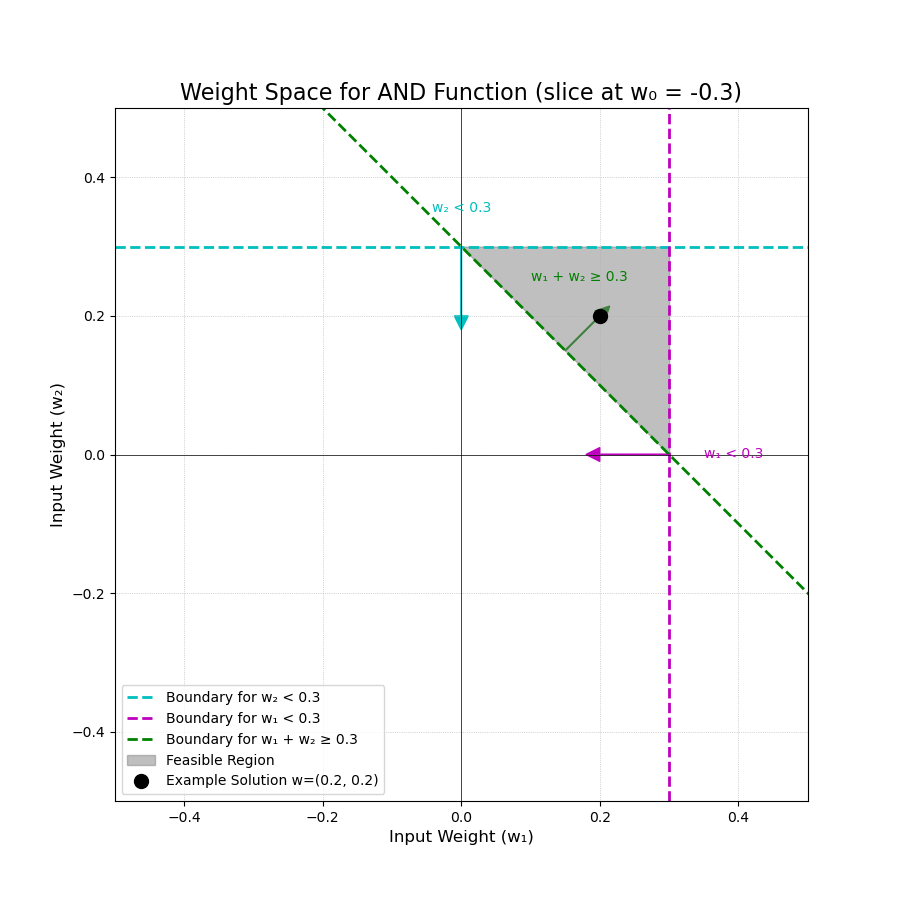
\includegraphics[width=0.6\textwidth]{and_weight_space.png}
    \caption{Weight space for the AND function using the bias trick. The feasible region is defined by the four constraints, and the point \(w_0 = -0.3\), \(w_1 = 0.2\), \(w_2 = 0.2\) is highlighted as an example.}
    \label{fig:and_weight_space}
\end{figure}

\section{Perceptron}

\section{The Perceptron: A Detailed Introduction}
The Perceptron is a simple binary classifier that serves as the foundational building block for more complex neural networks.

\begin{figure}
    \centering
    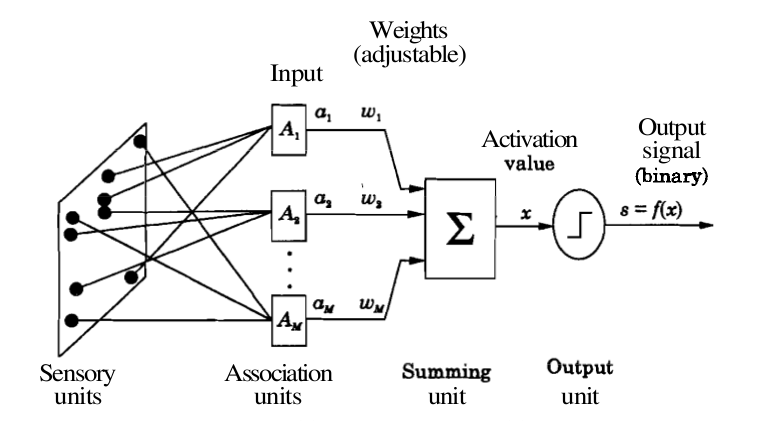
\includegraphics[width=0.6\textwidth]{perceptron.png}
    \caption{Architecture of a single-layer Perceptron. Inputs are weighted, summed, and passed through an activation function to produce the output.}
    \label{fig:perceptron_architecture} 
\end{figure}


\subsection{Definition: The Anatomy of a Perceptron}
For an input vector \(\mathbf{x} = (x_1, x_2, \dots, x_n)\), and the target vector \(\mathbf{t} = (t_1, t_2, \dots, t_n)\), the Perceptron computes a single output \(y\). This is done in two steps:
\begin{enumerate}
    \item \textbf{Compute a Weighted Sum:} The model calculates a weighted sum of the inputs, after the bias trick. This is the net input \(z\).
    \[ z = (w_1 x_1 + w_2 x_2 + \dots + w_n x_n) + b = \mathbf{w^{T}} \cdot \mathbf{x}\]
    \item \textbf{Apply an Activation Function:} The output \(z\) is passed through a Heaviside step function.
    \[ y = \phi(z) = \begin{cases} 1 & \text{if } z \ge 0 \\ 0 & \text{if } z < 0 \end{cases} \]
\end{enumerate}

\section{The Perceptron Learning Rule}
The Perceptron learns by adjusting its weights \(\mathbf{w}\) and bias \(b\) based on the errors it makes. This learning rule has strong theoretical foundations.
\begin{itemize}
    \item \textbf{Initialization}: Start with small random weights and bias.
    \item \textbf{Bias Trick}: Incorporate the bias into the weight vector by adding a dummy feature \(x_0 = 1\) and \(w_0\).
    \item \textbf{Learning Rate}: A small positive constant \(\eta\) controls the step size during weight updates.
    \item \textbf{Update Rule}: For each training example, update the weights and bias as follows:
    \item \textbf{Error Calculation}: Compute the error \(\epsilon = t - y\), where \(t\) is the true label.
    \item \textbf{Weight Update}: Adjust the weights and bias:
    \[ w_i \leftarrow w_i + \eta \cdot \epsilon \cdot x_i \quad \text{for all } i \]
    \[ b \leftarrow b + \eta \cdot \epsilon \]
    \item \textbf{Classification Condition}: The perceptron correctly classifies a training example \((\mathbf{x}^{(i)}, t^{(i)})\) if:
    \begin{itemize}
        \item If \(t^{(i)} = 1\) (positive class), then \(z^{(i)} > 0\)
        \item If \(t^{(i)} = 0\) (negative class), then \(z^{(i)} < 0\)
    \end{itemize}
    \item \textbf{Margin Condition}: To ensure robustness, we want training examples to be away from the decision boundary:
    \[ z^{(i)} \cdot t^{(i)} > 0 \]
      
\end{itemize}

\begin{block}{Note}
    If $\bm{x}^{(i)}$ is exactly on the decision boundary it will be classified as positive class. But we dont want our training examples to be on the decision boundary because a small noise or perturbation to the input features could change the classification. For robustness we want our training examples to be away from the decision boundary.
    \[z^{(i)} \cdot t^{(i)} > 0\]
\end{block}

\begin{fundasblock}{Functional Margin vs Geometric Margin}
\textbf{Functional Margin}:
\begin{itemize}
    \item The functional margin of a training example \((\mathbf{x}^{(i)}, t^{(i)})\) with respect to a weight vector \(\mathbf{w}\) is defined as:
    \[\hat{\gamma}^{(i)} = t^{(i)} (\mathbf{w}^T \mathbf{x}^{(i)})\]
    \item It measures how confidently the example is classified. A larger functional margin indicates a more confident classification.
    \item However, the functional margin is sensitive to the scale of the weight vector \(\mathbf{w}\). Scaling \(\mathbf{w}\) by a factor \(k\) scales the functional margin by the same factor \(k\).
    \item Thus, the functional margin does not provide a true measure of the distance from the decision boundary.
\end{itemize}
\end{fundasblock}



\subsection{The Perceptron Convergence Theorem: A Detailed Treatment}

\subsubsection{Introduction: A Fundamental Guarantee}

The \textbf{Perceptron Convergence Theorem} is a cornerstone of machine learning theory. It provides a simple but powerful promise: if your data can be separated by a line or plane (\textbf{linearly separable}), the Perceptron algorithm will find a solution in a \textbf{finite number of steps}. It proves that the algorithm doesn't just work by chance; it's guaranteed to succeed under the right conditions.

This section explores the proof of this theorem through three lenses: the rigorous algebra, the core intuition, and the elegant geometry.

\subsubsection{Convergence Theorem (Rosenblatt, 1962)}
\begin{theorem}[Perceptron Convergence]
If the training data is linearly separable, the perceptron learning algorithm will converge to a solution in a finite number of steps.
\end{theorem}

\subsubsection{The Formal Proof: An Algebraic Approach}

The proof ingeniously works by showing that two properties of the learning weight vector are on a collision course, forcing the process to end.

\textbf{The Setup:}
\begin{itemize}
    \item \textbf{Data}: A set of samples \(\{(\mathbf{x}_i, y_i)\}\), with labels \(y_i \in \{+1, -1\}\)
    \item \textbf{Assumption}: The data is \textbf{linearly separable}, meaning an ideal vector \(\mathbf{w}^*\) exists
    \item \textbf{Update Rule}: When a mistake occurs on point \(i\), the weight vector \(\mathbf{w}_k\) is updated: \(\mathbf{w}_{k+1} = \mathbf{w}_k + y_i \mathbf{x}_i\)
\end{itemize}

\textbf{Part 1: The Lower Bound (Steady Progress)}

This part shows that the weight vector \(\mathbf{w}_k\) gets progressively more \textbf{aligned} with the ideal vector \(\mathbf{w}^*\). We measure this alignment using the dot product.

\begin{block}{Key Formula 1: The Recursive Update}
\[\mathbf{w}_{k+1} \cdot \mathbf{w}^* \geq \mathbf{w}_k \cdot \mathbf{w}^* + \gamma\]
\end{block}

Here, \(\gamma\) is the \textbf{margin}, representing the "correctness score" of the point closest to the ideal hyperplane. Its existence is guaranteed by linear separability. After \(k\) updates:

\begin{block}{Key Result 1: The Lower Bound}
\[\mathbf{w}_k \cdot \mathbf{w}^* \geq k \gamma\]
\end{block}

This means the alignment with the correct solution grows steadily and linearly with every mistake.

\textbf{Part 2: The Upper Bound (Controlled Growth)}

This part shows that the vector's length is constrained and doesn't grow wildly. The squared magnitude of the weight vector is limited because the update rule includes a term that dampens its growth.

\begin{block}{Key Result 2: The Upper Bound}
\[||\mathbf{w}_k||^2 \leq k R^2\]
\end{block}

Where \(R^2\) is the squared magnitude of the largest input vector. This shows the squared length grows, at most, linearly with the number of mistakes.

\textbf{Part 3: The Contradiction}

We combine these two bounds using the \textbf{Cauchy-Schwarz inequality}, which states \((\mathbf{a} \cdot \mathbf{b})^2 \leq ||\mathbf{a}||^2 ||\mathbf{b}||^2\).

From Part 1, squaring both sides:
\[(\mathbf{w}_k \cdot \mathbf{w}^*)^2 \geq k^2\gamma^2\]

Applying Cauchy-Schwarz:
\[(\mathbf{w}_k \cdot \mathbf{w}^*)^2 \leq ||\mathbf{w}_k||^2 ||\mathbf{w}^*||^2\]

From Part 2, we know \(||\mathbf{w}_k||^2 \leq kR^2\), so:
\[(\mathbf{w}_k \cdot \mathbf{w}^*)^2 \leq kR^2 ||\mathbf{w}^*||^2\]

Combining the lower and upper bounds:
\[k^2\gamma^2 \leq (\mathbf{w}_k \cdot \mathbf{w}^*)^2 \leq kR^2 ||\mathbf{w}^*||^2\]

Simplifying:
\[k^2\gamma^2 \leq kR^2 ||\mathbf{w}^*||^2\]

Dividing by \(k\):
\[k\gamma^2 \leq R^2 ||\mathbf{w}^*||^2\]

\begin{block}{Final Result: The Bound on Mistakes}
\[k \leq \frac{R^2 ||\mathbf{w}^*||^2}{\gamma^2}\]
\end{block}

Since \(R\), \(||\mathbf{w}^*||\), and \(\gamma\) are all fixed, finite constants, this proves that the number of mistakes, \(k\), must be less than or equal to a finite number. \textbf{The contradiction arises if we assume the algorithm makes infinitely many mistakes}: the left side \(k\) would grow to infinity while the right side remains a fixed constant, which is impossible. Therefore, the algorithm must stop after a finite number of updates.

\subsubsection{Convergence Bound}
The perceptron will make at most \(\left(\frac{R}{\gamma}\right)^2\) mistakes, where:
\begin{itemize}
    \item \(R\) is the maximum norm of any training example: \(R = \max_i ||\mathbf{x}_i||\)
    \item \(\gamma\) is the margin of the optimal separating hyperplane
\end{itemize}

\begin{block}{Note on Normalization}
The general bound derived above is \(k \leq \frac{R^2 ||\mathbf{w}^*||^2}{\gamma^2}\). However, we can simplify this by normalizing \(\mathbf{w}^*\).

Since only the \textit{direction} of \(\mathbf{w}^*\) matters for classification (not its magnitude), we are free to normalize it to unit length: \(\|\mathbf{w}^*\| = 1\).

% If the original \(\mathbf{w}^*\) has norm \(\|\mathbf{w}^*\|\) and margin \(\gamma\), we can define:
% \[\tilde{\mathbf{w}}^* = \frac{\mathbf{w}^*}{\|\mathbf{w}^*\|}, \quad \tilde{\gamma} = \frac{\gamma}{\|\mathbf{w}^*\|}\]

% Then \(\|\tilde{\mathbf{w}}^*\| = 1\) and the bound becomes:
% \[k \leq \frac{R^2 \|\tilde{\mathbf{w}}^*\|^2}{\tilde{\gamma}^2} = \frac{R^2 \cdot 1}{\left(\frac{\gamma}{\|\mathbf{w}^*\|}\right)^2} = \frac{R^2 \|\mathbf{w}^*\|^2}{\gamma^2}\]

When we assume \(\mathbf{w}^*\) is already normalized (the standard convention), the bound simplifies to \(\left(\frac{R}{\gamma}\right)^2\).
\end{block}

\subsubsection{The Geometric Interpretation: The Cone and The Sphere}

The algebra tells a beautiful geometric story. The proof traps the learning vector in a "squeeze play."

\begin{itemize}
    \item \textbf{The Cone of Progress}: The lower bound forces the angle between our vector \(\mathbf{w}_k\) and the ideal vector \(\mathbf{w}^*\) to get smaller with every mistake. This confines \(\mathbf{w}_k\) to an ever-narrowing \textbf{cone}.

    \item \textbf{The Sphere of Possibility}: The upper bound forces the tip of the vector \(\mathbf{w}_k\) to stay inside a \textbf{sphere} whose radius grows slowly (with \(\sqrt{k}\)).
\end{itemize}

\textbf{The Contradiction}: The cone narrows faster than the sphere expands. Eventually, the cone becomes so tight that any vector that could fit inside it would have to be longer than the radius of the allowed sphere. The geometric constraints become impossible to satisfy, proving the process must end.

\begin{figure}[h]
    \centering
    \href{https://youtu.be/lBzRw57xI9o}{
        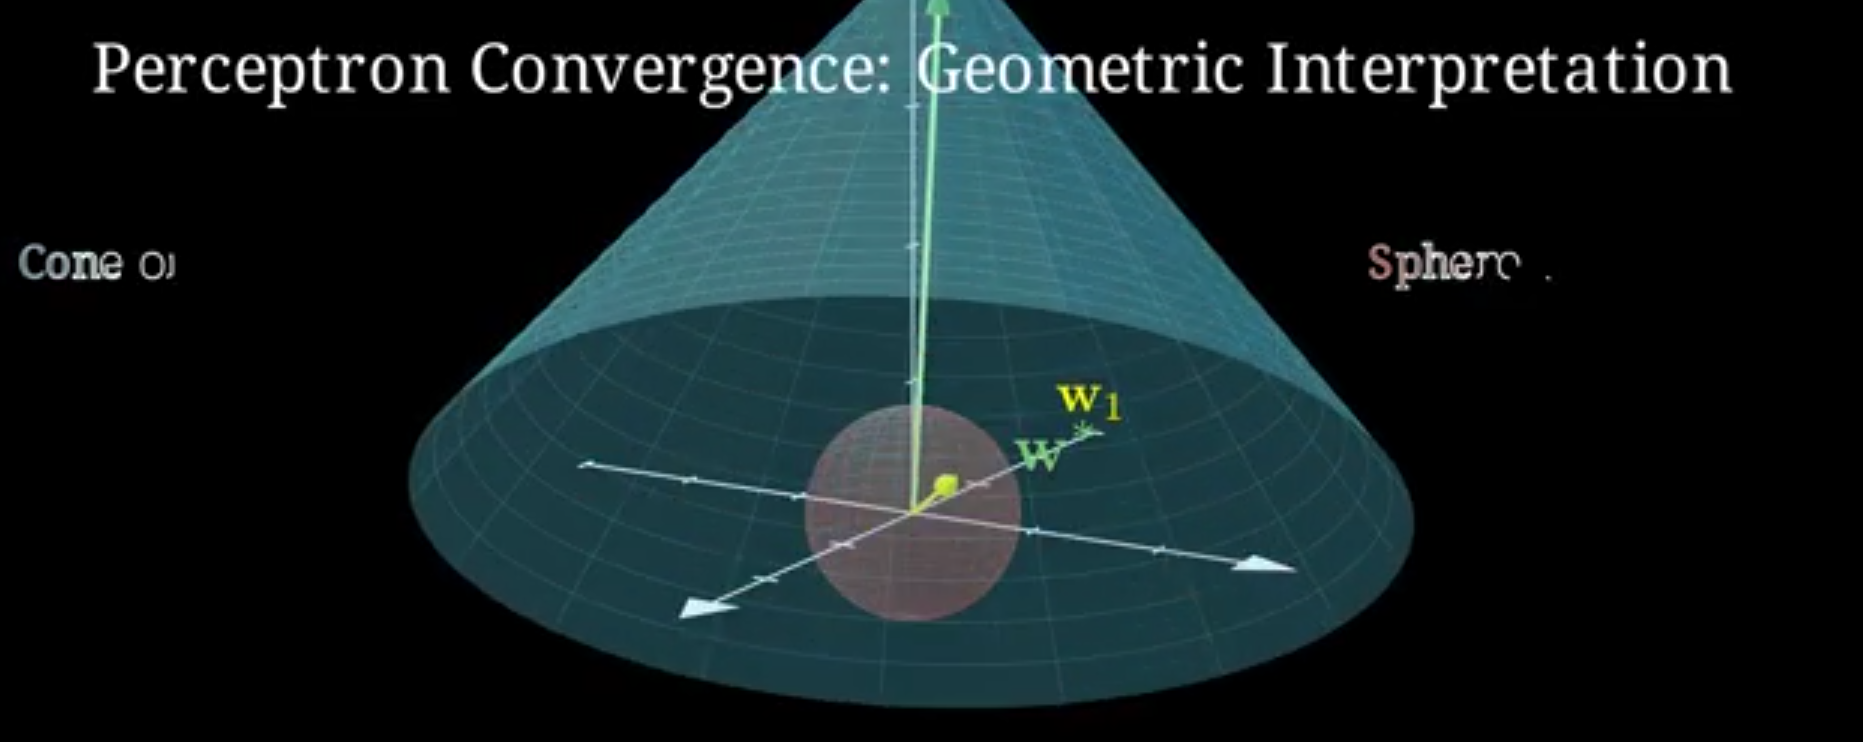
\includegraphics[width=0.6\textwidth]{youtube_thumbnail.png}
    }
    \caption{Geometric interpretation of Perceptron convergence. Click to view video on YouTube.}
    \label{fig:perceptron_convergence_video}
\end{figure}

\subsubsection{Relevance in Modern Deep Learning}

Understanding this theorem is more than a historical exercise. It teaches foundational principles that are still relevant today:

\begin{itemize}
    \item \textbf{Intuition for Optimization}: It provides a mental model for how algorithms navigate a solution space
    \item \textbf{Basis for Advanced Concepts}: The concept of a \textbf{margin} (\(\gamma\)) is central to more advanced and powerful algorithms like Support Vector Machines (SVMs)
    \item \textbf{Theoretical Rigor}: It's a perfect example of how to formally reason about an algorithm's behavior, a skill essential for creating new methods
\end{itemize}

\section{Optimal Separating Hyperplane and Margin Theory}

\subsection{The Optimal Weight Vector \(\mathbf{w}^*\)}

The foundation of perceptron convergence theory rests on the existence of an optimal weight vector \(\mathbf{w}^*\) that not only correctly classifies all training examples but does so with a guaranteed minimum margin.

\begin{definition}[Optimal Separating Hyperplane]
For a linearly separable dataset \(\{(\mathbf{x}_i, y_i)\}_{i=1}^N\) where \(y_i \in \{-1, +1\}\), an optimal weight vector \(\mathbf{w}^*\) is one that correctly classifies all training examples with margin \(\gamma > 0\):
\[y_i(\mathbf{w}^{*T} \mathbf{x}_i) \geq \gamma \quad \forall i \in \{1, 2, \ldots, N\}\]
\end{definition}

\subsection{Understanding the Margin Condition}

\subsubsection{Mathematical Interpretation}
The condition \(y_i(\mathbf{w}^{*T} \mathbf{x}_i) \geq \gamma\) encodes several crucial properties:

\begin{itemize}
    \item \textbf{Correct Classification}: Since \(y_i \in \{-1, +1\}\) and \(\gamma > 0\), the product \(y_i(\mathbf{w}^{*T} \mathbf{x}_i)\) must be positive, ensuring correct classification
    \item \textbf{Confidence Measure}: The magnitude \(|\mathbf{w}^{*T} \mathbf{x}_i|\) represents the "confidence" of classification
    \item \textbf{Minimum Separation}: The margin \(\gamma\) ensures all points are at least a minimum distance from the decision boundary
\end{itemize}

\subsubsection{Geometric Interpretation}
\begin{itemize}
    \item \textbf{Positive Examples} (\(y_i = +1\)): Must satisfy \(\mathbf{w}^{*T} \mathbf{x}_i \geq \gamma\)
    \item \textbf{Negative Examples} (\(y_i = -1\)): Must satisfy \(\mathbf{w}^{*T} \mathbf{x}_i \leq -\gamma\)
    \item \textbf{Decision Boundary}: The hyperplane \(\mathbf{w}^{*T} \mathbf{x} = 0\)
    \item \textbf{Margin Boundaries}: Hyperplanes \(\mathbf{w}^{*T} \mathbf{x} = \pm\gamma\)
\end{itemize}

\section{Optimal Margin Computation: A Glimpse of SVM}

In linear classification, the concept of an \textbf{optimal margin} is central to robust decision boundaries. The optimal margin is the largest possible distance between the decision boundary and the closest data points from each class. These closest points are known as \textit{support vectors}.

\subsection{Algorithm Overview}

\begin{enumerate}
    \item \textbf{Identify Support Vectors}: For two linearly separable classes, find the pair of points (one from each class) that are closest to each other.
        \item \textbf{Compute Direction}: The vector connecting these support vectors defines the orientation of the optimal separating hyperplane.
        \item \textbf{Place the Decision Boundary}: Position the decision boundary halfway between the support vectors, perpendicular to the direction vector.
        \item \textbf{Calculate the Margin}: The margin is half the distance between the support vectors, measured along the direction vector.
        \item \textbf{Visualize}: The margin boundaries are parallel to the decision boundary and pass through the support vectors (refer to figure \ref{fig:optimal_margin_glimpse}).
\end{enumerate}
\begin{figure}[htbp]
    \centering
    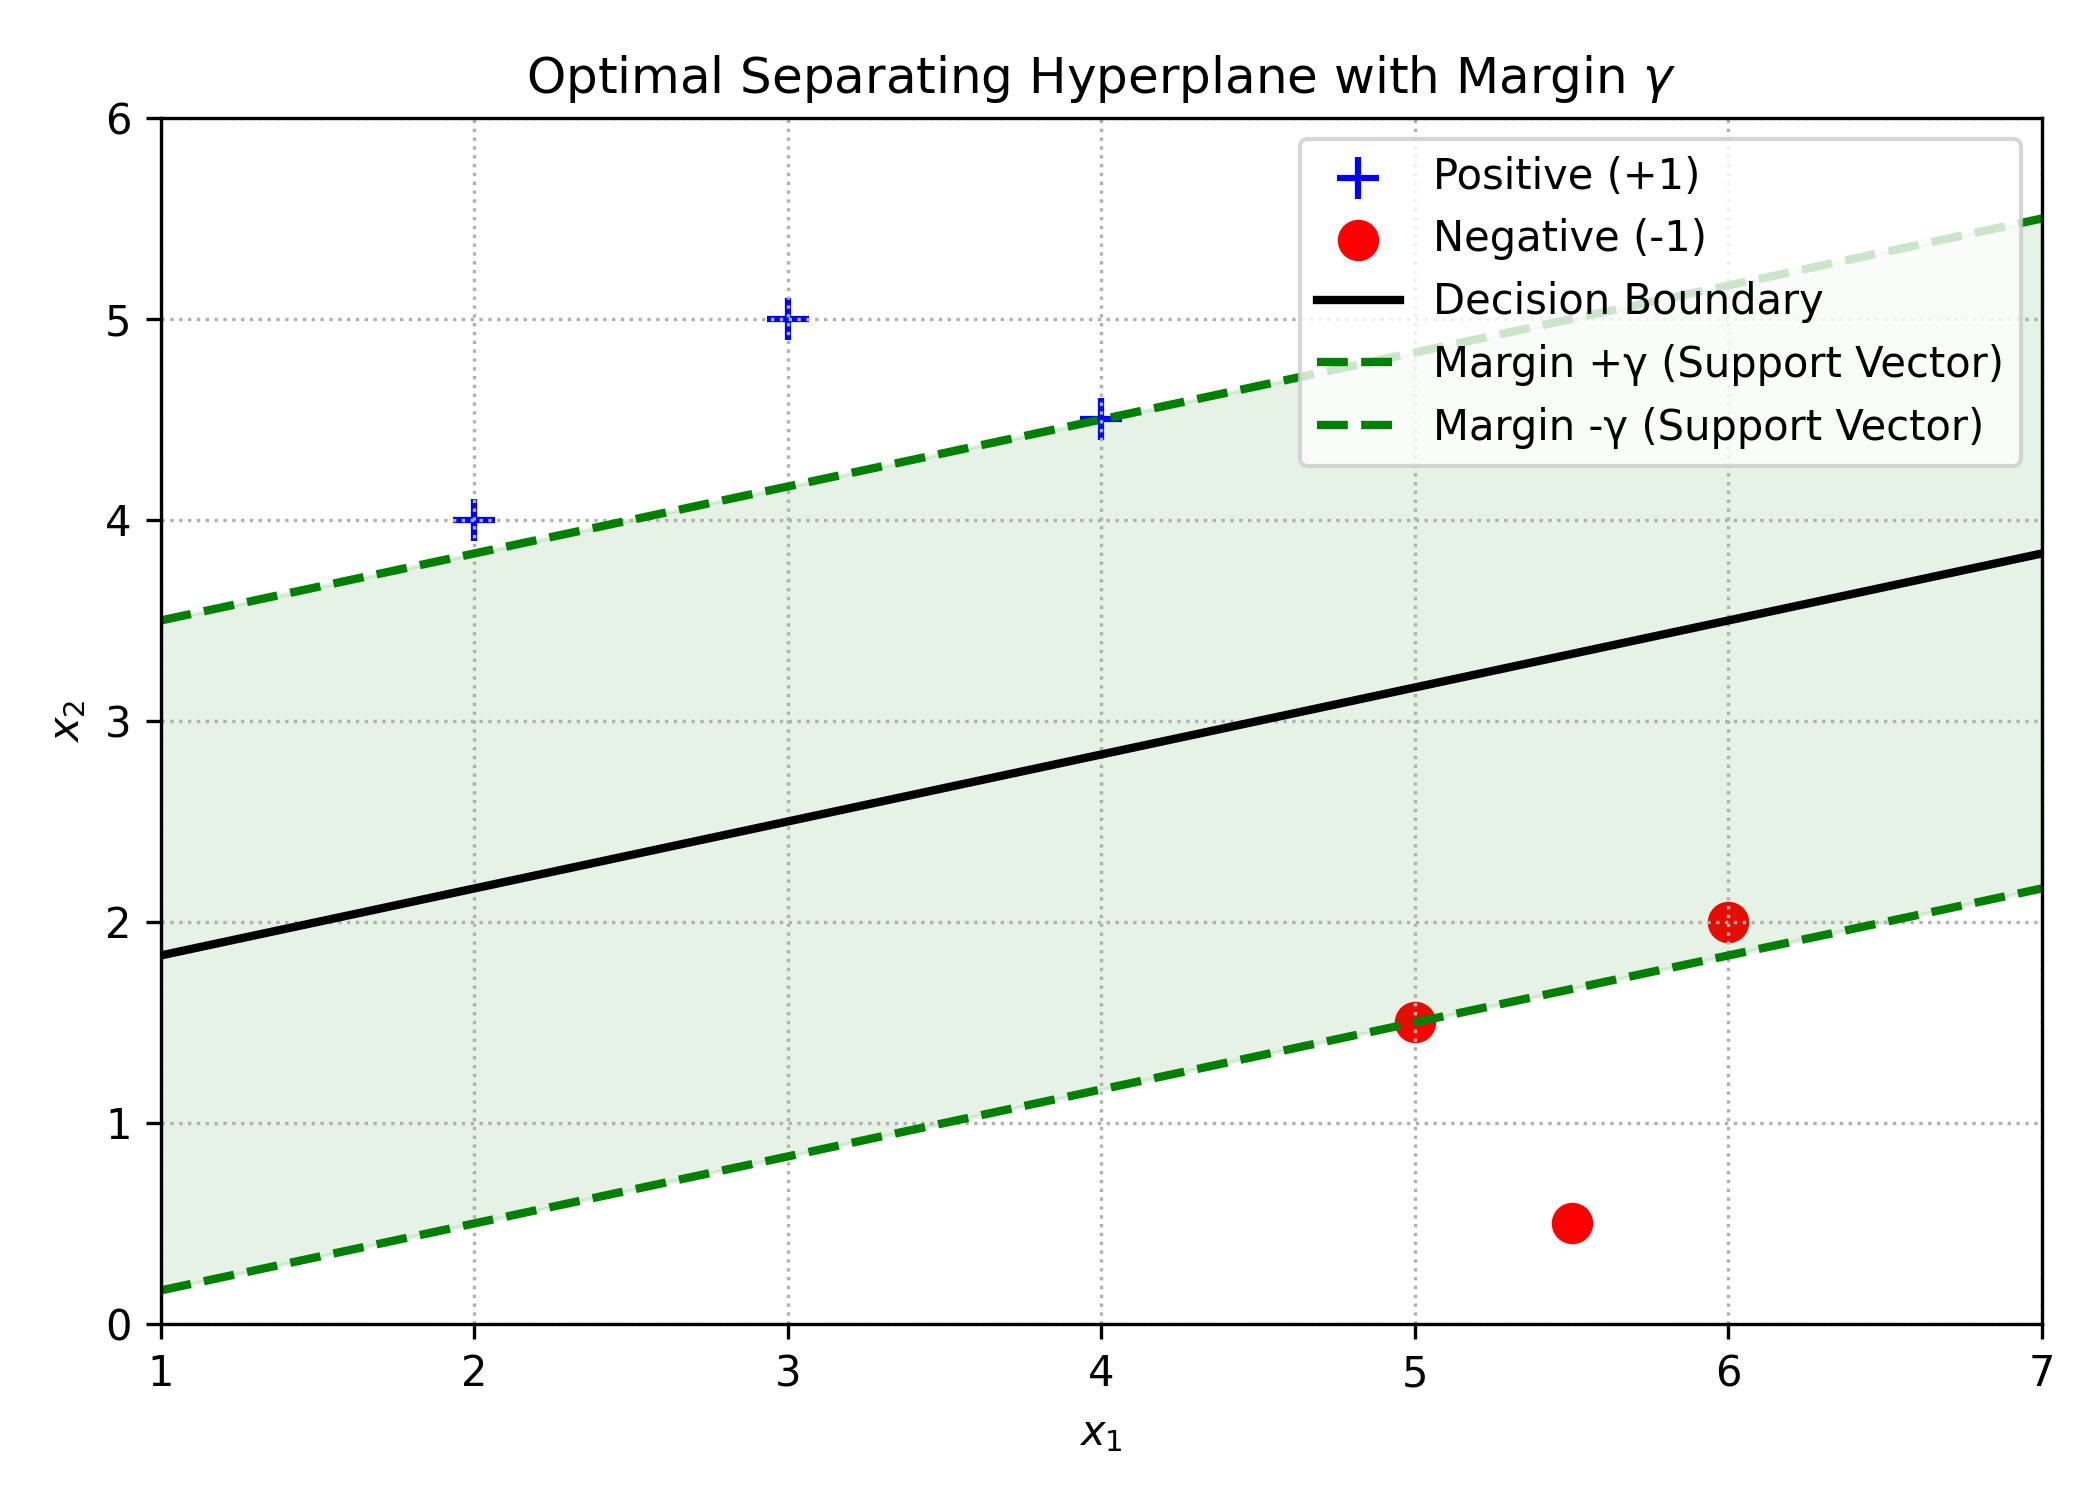
\includegraphics[width=0.8\textwidth]{optimal_margin.png}
    \caption{Optimal margin computation: The decision boundary is placed halfway between the closest points (support vectors) of each class, maximizing the margin.}
    \label{fig:optimal_margin_glimpse}
\end{figure}
\subsection{Why Is This Important?}

Maximizing the margin leads to better generalization and robustness against noise. This principle is the foundation of \textbf{Support Vector Machines (SVMs)}, which explicitly seek the hyperplane with the largest margin. While SVMs use more advanced optimization techniques, the geometric intuition shown here provides a glimpse into their core idea.




\subsection{The Role of Normalization}

\subsubsection{Functional vs. Geometric Margin}
The margin \(\gamma\) in our definition is the \textbf{functional margin}. To obtain the \textbf{geometric margin} (actual distance), we need normalization:

\begin{definition}[Geometric Margin]
The geometric margin is the actual perpendicular distance from training examples to the decision boundary:
\[\gamma_{\text{geom}} = \frac{\gamma}{||\mathbf{w}^*||_2}\]
\end{definition}

\subsubsection{Canonical Form}
We can always normalize \(\mathbf{w}^*\) such that the functional margin equals 1:
\[\tilde{\mathbf{w}}^* = \frac{\mathbf{w}^*}{\gamma}, \quad \text{giving} \quad y_i(\tilde{\mathbf{w}}^{*T} \mathbf{x}_i) \geq 1 \quad \forall i\]

\subsection{Existence and Uniqueness}

\subsubsection{Existence Condition}
\begin{theorem}[Existence of Optimal Separator]
For a linearly separable dataset, there always exists at least one weight vector \(\mathbf{w}^*\) with margin \(\gamma > 0\) that correctly classifies all training examples.
\end{theorem}

\begin{proof}[Proof Sketch]
If the dataset is linearly separable, then there exists some \(\mathbf{w}_0\) such that \(y_i(\mathbf{w}_0^T \mathbf{x}_i) > 0\) for all \(i\). Since there are finitely many training examples, we can define:
\[\gamma = \min_{i=1}^N y_i(\mathbf{w}_0^T \mathbf{x}_i) > 0\]
Thus, \(\mathbf{w}^* = \mathbf{w}_0\) satisfies our condition.
\end{proof}

\subsubsection{Non-Uniqueness}
The optimal weight vector \(\mathbf{w}^*\) is generally \textbf{not unique}:
\begin{itemize}
    \item Any positive scalar multiple \(c\mathbf{w}^*\) (where \(c > 0\)) also satisfies the condition with margin \(c\gamma\)
    \item Different weight vectors may achieve different margins
    \item The perceptron algorithm finds \textit{any} separating hyperplane, not necessarily the optimal one
\end{itemize}

\subsection{Connection to Perceptron Convergence}

\subsubsection{The Convergence Theorem Framework}
The existence of \(\mathbf{w}^*\) with margin \(\gamma\) is crucial for proving perceptron convergence as we ssaw from the perceptron convergence theorem:
\subsection{Practical Implications}

\subsubsection{Algorithm Design}
Understanding the optimal separator helps in:
\begin{itemize}
    \item \textbf{Convergence Analysis}: Predicting how long training will take
    \item \textbf{Learning Rate Selection}: Choosing appropriate step sizes
    \item \textbf{Initialization Strategies}: Starting with reasonable weight vectors
\end{itemize}

\subsubsection{Dataset Assessment}
The margin \(\gamma\) provides insights about the dataset:
\begin{itemize}
    \item \textbf{Large \(\gamma\)}: Easy problem, fast convergence expected
    \item \textbf{Small \(\gamma\)}: Difficult problem, slow convergence, sensitive to noise
    \item \textbf{No \(\gamma > 0\)}: Dataset is not linearly separable
\end{itemize}

\subsection{Example: Optimal Separator for AND Function}

Let's find the optimal weight vector for the AND function with margin analysis.

\subsubsection{Training Data}
Using the augmented representation (bias trick):
\[
X = \begin{pmatrix}
1 & 0 & 0 \\
1 & 0 & 1 \\
1 & 1 & 0 \\
1 & 1 & 1
\end{pmatrix}, \quad
y = \begin{pmatrix}
-1 \\
-1 \\
-1 \\
+1
\end{pmatrix}
\]

\subsubsection{Finding the Optimal Separator}
We need to find \(\mathbf{w}^* = [w_0, w_1, w_2]^T\) such that:
\begin{align}
y_1(\mathbf{w}^{*T} \mathbf{x}_1) = -1(w_0) &\geq \gamma \\
y_2(\mathbf{w}^{*T} \mathbf{x}_2) = -1(w_0 + w_2) &\geq \gamma \\
y_3(\mathbf{w}^{*T} \mathbf{x}_3) = -1(w_0 + w_1) &\geq \gamma \\
y_4(\mathbf{w}^{*T} \mathbf{x}_4) = +1(w_0 + w_1 + w_2) &\geq \gamma
\end{align}

\subsubsection{Solution with Maximum Margin}
To find the maximum margin solution, we solve:
\begin{align}
-w_0 &\geq \gamma \\
-w_0 - w_2 &\geq \gamma \\
-w_0 - w_1 &\geq \gamma \\
w_0 + w_1 + w_2 &\geq \gamma
\end{align}

Setting all inequalities to equality for the maximum margin:
\[w_0 = -\gamma, \quad w_1 = w_2 = 0, \quad \text{but this violates the fourth constraint}\]

The actual maximum margin solution requires solving a quadratic programming problem, yielding approximately:
\[\mathbf{w}^* = [-0.5, 0.5, 0.5]^T \quad \text{with} \quad \gamma = 0.5\]

This gives us the decision boundary \(-0.5 + 0.5x_1 + 0.5x_2 = 0\), or equivalently \(x_1 + x_2 = 1\).

\subsection{Learning Rate Analysis}
\subsubsection{Effect of Learning Rate \(\eta\)}
\begin{itemize}
    \item \textbf{Large \(\eta\)}: Faster convergence but may overshoot optimal solution
    \item \textbf{Small \(\eta\)}: More stable learning but slower convergence
    \item \textbf{Theoretical Result}: For linearly separable data, any \(\eta > 0\) guarantees convergence
\end{itemize}

\subsubsection{Adaptive Learning Rates}
Common strategies include:
\begin{itemize}
    \item \textbf{Time decay}: \(\eta_t = \frac{\eta_0}{1 + \alpha t}\)
    \item \textbf{Step decay}: Reduce \(\eta\) by factor every few epochs
    \item \textbf{Performance-based}: Reduce \(\eta\) when performance plateaus
\end{itemize}

\section{Vectorisation of Perceptron Learning Rule: A Matrix-Based Example}
To see how vectorization works in practice, let's walk through the process using a full matrix-based approach for the AND function. This method calculates the updates for all samples in the dataset (a "batch") and then applies a single, consolidated update at the end of the epoch.

\subsection{Mathematical Foundation of Vectorization}
Vectorization allows us to process multiple training examples simultaneously using matrix operations instead of iterating through samples one by one. This approach is:
\begin{itemize}
    \item \textbf{Computationally efficient}: Modern hardware (GPUs) excels at matrix operations
    \item \textbf{Mathematically elegant}: Compact representation of batch operations
    \item \textbf{Numerically stable}: Reduces accumulated floating-point errors
\end{itemize}

\subsection{Define the Matrices}
For the AND function, we use an augmented Input Matrix \(X\), a Weight Vector \(W\), and a Target Vector \(T\).

\subsubsection{Input Matrix \(X\) (Augmented Design Matrix)}
The input matrix includes a bias column (first column of 1s) followed by the feature columns:
\[
X = \begin{pmatrix}
1 & 0 & 0 \\
1 & 0 & 1 \\
1 & 1 & 0 \\
1 & 1 & 1
\end{pmatrix}_{4 \times 3}
\]
where:
\begin{itemize}
    \item Rows represent training examples (4 samples)
    \item First column represents bias input (always 1)
    \item Remaining columns represent feature inputs \(x_1, x_2\)
\end{itemize}

\subsubsection{Target Vector \(T\)}
\[
T = \begin{pmatrix}
0 \\
0 \\
0 \\
1
\end{pmatrix}_{4 \times 1}
\]

\subsubsection{Weight Vector \(W\)}
Let's initialize the weight vector \(W\) to zeros and use a learning rate \(\eta = 0.1\).
\[
W_0 = \begin{pmatrix}
w_0 \\
w_1 \\
w_2
\end{pmatrix} = \begin{pmatrix}
0 \\
0 \\
0
\end{pmatrix}_{3 \times 1}
\]
where \(w_0\) is the bias weight, \(w_1\) and \(w_2\) are feature weights.

\subsection{Epoch 1: Mathematical Flow}
\subsubsection{Step 1: Compute Net Input Z}
The net input is computed as \(Z = X \cdot W\), where we multiply the \(4 \times 3\) input matrix by the \(3 \times 1\) weight vector to get a \(4 \times 1\) output vector.
\[
Z = X \cdot W_0 = \begin{pmatrix}
1 & 0 & 0 \\
1 & 0 & 1 \\
1 & 1 & 0 \\
1 & 1 & 1
\end{pmatrix}_{4 \times 3} \begin{pmatrix}
0 \\
0 \\
0
\end{pmatrix}_{3 \times 1} = \begin{pmatrix}
1 \cdot 0 + 0 \cdot 0 + 0 \cdot 0 \\
1 \cdot 0 + 0 \cdot 0 + 1 \cdot 0 \\
1 \cdot 0 + 1 \cdot 0 + 0 \cdot 0 \\
1 \cdot 0 + 1 \cdot 0 + 1 \cdot 0
\end{pmatrix} = \begin{pmatrix}
0 \\
0 \\
0 \\
0
\end{pmatrix}_{4 \times 1}
\]

\textbf{Matrix Dimension Check:} \((4 \times 3) \times (3 \times 1) = (4 \times 1)\) 

\subsubsection{Step 2: Apply Activation Function to get Output Y}
Apply the Heaviside step function element-wise: \(\phi(z) = \begin{cases} 1 & \text{if } z \geq 0 \\ 0 & \text{if } z < 0 \end{cases}\)
\[
Y = \phi(Z) = \phi \begin{pmatrix}
0 \\
0 \\
0 \\
0
\end{pmatrix}_{4 \times 1} = \begin{pmatrix}
\phi(0) \\
\phi(0) \\
\phi(0) \\
\phi(0)
\end{pmatrix} = \begin{pmatrix}
1 \\
1 \\
1 \\
1
\end{pmatrix}_{4 \times 1}
\]
Since all net inputs are 0, and \(\phi(0) = 1\) by our step function definition, all outputs are 1.

\subsubsection{Step 3: Calculate the Error Vector E}
\[
E = T - Y =
\begin{pmatrix}
0 \\
0 \\
0 \\
1
\end{pmatrix}
-
\begin{pmatrix}
1 \\
1 \\
1 \\
1
\end{pmatrix}
=
\begin{pmatrix}
-1 \\
-1 \\
-1 \\
0
\end{pmatrix}
\]

\subsubsection{Step 4: Calculate the Total Weight Update \(\Delta W\)}
The weight update is computed as \(\Delta W = \eta \cdot (X^T \cdot E)\), where we multiply the transpose of the input matrix by the error vector.

First, let's compute \(X^T\):
\[
X^T = \begin{pmatrix}
1 & 0 & 0 \\
1 & 0 & 1 \\
1 & 1 & 0 \\
1 & 1 & 1
\end{pmatrix}^T = \begin{pmatrix}
1 & 1 & 1 & 1 \\
0 & 0 & 1 & 1 \\
0 & 1 & 0 & 1
\end{pmatrix}_{3 \times 4}
\]

Now compute the weight update:
\[
\Delta W = \eta \cdot (X^T \cdot E) = 0.1 \cdot \begin{pmatrix}
1 & 1 & 1 & 1 \\
0 & 0 & 1 & 1 \\
0 & 1 & 0 & 1
\end{pmatrix}_{3 \times 4} \begin{pmatrix}
-1 \\
-1 \\
-1 \\
0
\end{pmatrix}_{4 \times 1}
\]

\[
= 0.1 \cdot \begin{pmatrix}
1(-1) + 1(-1) + 1(-1) + 1(0) \\
0(-1) + 0(-1) + 1(-1) + 1(0) \\
0(-1) + 1(-1) + 0(-1) + 1(0)
\end{pmatrix} = 0.1 \cdot \begin{pmatrix}
-3 \\
-1 \\
-1
\end{pmatrix} = \begin{pmatrix}
-0.3 \\
-0.1 \\
-0.1
\end{pmatrix}_{3 \times 1}
\]

\textbf{Matrix Dimension Check:} \((3 \times 4) \times (4 \times 1) = (3 \times 1)\) 

\subsubsection{Step 5: Update the Weight Vector W}
\[
W_1 = W_0 + \Delta W =
\begin{pmatrix}
0 \\
0 \\
0
\end{pmatrix}
+
\begin{pmatrix}
-0.3 \\
-0.1 \\
-0.1
\end{pmatrix}
=
\begin{pmatrix}
-0.3 \\
-0.1 \\
-0.1
\end{pmatrix}
\]
After the first epoch, our new weight vector is \(W_1 = (-0.3, -0.1, -0.1)^T\).



\section{Limitations of Linear Classifiers}

\subsection{Linear Separability}

\begin{definition}[Linear Separability]
A dataset is linearly separable if there exists a linear decision boundary that perfectly separates the two classes.
\end{definition}

\subsection{Convexity and Separability}

\begin{definition}[Convex Set]
A set is convex if the line segment between any two points in the set lies entirely within the set.
\end{definition}

\begin{theorem}[Linear Separability Condition]
If the positive examples form a convex set and the negative examples form a convex set, and these sets do not overlap, then the data is linearly separable.
\end{theorem}

\subsection{The XOR Problem}

\textbf{XOR Truth Table}: $(0,0) \rightarrow 0$, $(0,1) \rightarrow 1$, $(1,0) \rightarrow 1$, $(1,1) \rightarrow 0$

\textbf{Why XOR is not linearly separable}:
\begin{itemize}
    \item Positive examples: $(0,1)$ and $(1,0)$
    \item Negative examples: $(0,0)$ and $(1,1)$
    \item No single line can separate these points correctly
\end{itemize}

\subsection{Overcoming Limitations: Basis Functions}

\textbf{Strategy}: Transform inputs using basis functions $\bm{\phi}(\bm{x})$ to create a new feature space where linear separation becomes possible.

\textbf{Example for XOR}:
\begin{itemize}
    \item Original features: $x_1, x_2$
    \item Basis functions: $\phi_1 = x_1$, $\phi_2 = x_2$, $\phi_3 = x_1 x_2$
    \item In the new space $[x_1, x_2, x_1 x_2]$, XOR becomes linearly separable
\end{itemize}

The transformed XOR problem becomes:
\begin{align}
(0,0,0) &\rightarrow 0 \\
(0,1,0) &\rightarrow 1 \\
(1,0,0) &\rightarrow 1 \\
(1,1,1) &\rightarrow 0
\end{align}

With weights $w_1 = 1$, $w_2 = 1$, $w_3 = -2$, and bias $b = -0.5$:
\begin{equation}
\hat{y} = 1 \text{ if } x_1 + x_2 - 2x_1x_2 - 0.5 > 0
\end{equation}

\section{Practical Considerations}

\subsection{Feature Engineering}
\begin{itemize}
    \item \textbf{Normalization}: Scale features to similar ranges
    \item \textbf{Interaction terms}: Add products of features $(x_1 x_2)$
    \item \textbf{Polynomial features}: Add powers of features $(x_1^2, x_2^2)$
\end{itemize}

\subsection{Model Selection}
\begin{itemize}
    \item \textbf{Bias-variance tradeoff}: Simple models (few features) vs. complex models (many features)
    \item \textbf{Interpretability}: Linear classifiers provide clear feature importance through weights
    \item \textbf{Computational efficiency}: Linear models are fast to train and evaluate
\end{itemize}

\subsection{Performance Evaluation}
\begin{itemize}
    \item \textbf{Training accuracy}: Percentage of training examples correctly classified
    \item \textbf{Generalization}: Performance on unseen test data
    \item \textbf{Decision boundary visualization}: Plot boundaries in 2D for intuition
\end{itemize}

\section{Limitations of the Perceptron}
\subsection{Linear Separability Constraint}
The fundamental limitation of the perceptron is that it can only learn linearly separable functions.

\subsubsection{Definition: Linear Separability}
A dataset is \textbf{linearly separable} if there exists a hyperplane that perfectly separates the positive and negative examples:
\[\exists \mathbf{w}, b : y_i(\mathbf{w}^T \mathbf{x}_i + b) > 0 \quad \forall i\]

\subsubsection{The XOR Problem (Minsky \& Papert, 1969)}
Consider the XOR function:
\begin{center}
\begin{tabular}{|c|c|c|}
\hline
\(x_1\) & \(x_2\) & XOR \\
\hline
0 & 0 & 0 \\
0 & 1 & 1 \\
1 & 0 & 1 \\
1 & 1 & 0 \\
\hline
\end{tabular}
\end{center}

\textbf{Mathematical Proof of Non-Linear Separability}:
Assume there exists a linear classifier \(\mathbf{w}^T \mathbf{x} + b = 0\) that separates XOR data.
For the four points, we need:
\begin{align}
w_1 \cdot 0 + w_2 \cdot 0 + b &< 0 \quad \text{(point (0,0))} \\
w_1 \cdot 0 + w_2 \cdot 1 + b &> 0 \quad \text{(point (0,1))} \\
w_1 \cdot 1 + w_2 \cdot 0 + b &> 0 \quad \text{(point (1,0))} \\
w_1 \cdot 1 + w_2 \cdot 1 + b &< 0 \quad \text{(point (1,1))}
\end{align}

From equations (1) and (2): \(b < 0\) and \(w_2 + b > 0 \Rightarrow w_2 > -b > 0\)
From equations (1) and (3): \(b < 0\) and \(w_1 + b > 0 \Rightarrow w_1 > -b > 0\)
From equation (4): \(w_1 + w_2 + b < 0\)

But this contradicts \(w_1 > -b\) and \(w_2 > -b\), since:
\[w_1 + w_2 + b > -b + (-b) + b = -b > 0\]

Therefore, no linear separator exists for XOR.

\subsection{Solutions to Linear Separability Limitation}
\subsubsection{Multi-Layer Perceptrons (MLPs)}
\begin{itemize}
    \item Add hidden layers with non-linear activation functions
    \item Can approximate any continuous function (Universal Approximation Theorem)
    \item Require more sophisticated training algorithms (backpropagation)
\end{itemize}

\subsubsection{Feature Engineering}
\begin{itemize}
    \item Transform input space to make data linearly separable
    \item For XOR: Add feature \(x_3 = x_1 \oplus x_2\) (though this requires knowing the solution)
    \item Kernel methods: Implicitly map to higher-dimensional spaces
\end{itemize}

\subsubsection{Ensemble Methods}
\begin{itemize}
    \item Combine multiple linear classifiers
    \item Voting or weighted combination schemes
    \item Can learn non-linear decision boundaries
\end{itemize}

\section{Historical Impact and Legacy}
\subsection{The Perceptron Controversy}
The 1969 book "Perceptrons" by Minsky and Papert highlighted the limitations of single-layer perceptrons, leading to:
\begin{itemize}
    \item \textbf{AI Winter}: Reduced funding and interest in neural networks
    \item \textbf{Focus shift}: Emphasis moved to symbolic AI and expert systems
    \item \textbf{Delayed progress}: Multi-layer networks existed but lacked efficient training methods
\end{itemize}

\subsection{Modern Relevance}
Despite limitations, perceptrons remain important because:
\begin{itemize}
    \item \textbf{Building blocks}: Neurons in modern deep networks are perceptron variants
    \item \textbf{Theoretical foundation}: Understanding linear classifiers is crucial
    \item \textbf{Computational efficiency}: Still useful for linearly separable problems
    \item \textbf{Online learning}: Perceptron learning rule works in streaming settings
\end{itemize}

\section{Exercises} 
 
\begin{enumerate}
    \item Determine the weights of a network with 4 input and 2 output units using Perceptron learning law
\end{enumerate}
Input:
\(\begin{pmatrix} 1 & 1 & 0 & 0 \\ 1 & 0 & 0 & 1 \\ 0 & 0 & 1 & 1 \\ 0 & 1 & 1 & 0 \end{pmatrix}\)
Output:
\( \begin{pmatrix} 1& 1 & 1 & 0 & 0 \end{pmatrix} \)

\section{Chapter Summary}

This chapter provided a comprehensive introduction to linear classification, covering both theoretical foundations and practical implementations. The key concepts and contributions include:

\subsection{Foundational Concepts}
\begin{enumerate}
    \item \textbf{Binary Linear Classification Framework}: Established the mathematical foundation using hyperplanes as decision boundaries, with clear geometric interpretation in both input and weight spaces.
    
    \item \textbf{Bias-Threshold Elimination}: Demonstrated how redundant parameters can be eliminated using the "bias trick" with dummy features, simplifying the mathematical representation.
    
    \item \textbf{Geometric Duality}: Explored the relationship between input space (where data points and decision boundaries exist) and weight space (where constraints from training examples define feasible regions).
\end{enumerate}

\subsection{The Perceptron Algorithm}
\begin{enumerate}
    \item \textbf{Mathematical Definition}: Introduced the perceptron as a linear classifier with step activation function, providing the complete mathematical formulation.
    
    \item \textbf{Learning Rule}: Derived the perceptron learning algorithm with convergence guarantees for linearly separable data (Rosenblatt's Convergence Theorem).
    
    \item \textbf{Vectorization}: Presented efficient matrix-based implementations for batch processing, demonstrating how modern computational approaches handle multiple training examples simultaneously.
\end{enumerate}

\subsection{Practical Applications and Examples}
\begin{enumerate}
    \item \textbf{Logic Functions}: Worked through concrete examples (NOT, AND gates) showing how to derive weights systematically and visualize solutions in both input and weight spaces.
    
    \item \textbf{Computational Implementation}: Provided detailed mathematical flows for vectorized perceptron learning with step-by-step matrix calculations.
    
    \item \textbf{Real-world Context}: Connected theoretical concepts to practical applications in medical diagnosis, spam detection, and fraud prevention.
\end{enumerate}

\subsection{Limitations and Extensions}
\begin{enumerate}
    \item \textbf{Linear Separability Constraint}: Analyzed fundamental limitations through the XOR problem, providing mathematical proof of non-separability.
    
    \item \textbf{Solution Strategies}: Introduced approaches to overcome limitations including basis functions, multi-layer perceptrons, and feature engineering.
    
    \item \textbf{Historical Context}: Discussed the impact of early limitations on the field's development and the subsequent renaissance of neural networks.
\end{enumerate}

\subsection{Key Mathematical Results}
\begin{itemize}
    \item \textbf{Convergence Bound}: The perceptron makes at most $\left(\frac{R}{\gamma}\right)^2$ mistakes for linearly separable data
    \item \textbf{Geometric Margin}: Distance from hyperplane to data points quantifies classification confidence
    \item \textbf{Feasible Region}: Intersection of half-spaces in weight space defines all valid solutions
\end{itemize}

\subsection{Computational Insights}
The chapter demonstrated how theoretical concepts translate to practical implementations:
\begin{itemize}
    \item Matrix operations enable efficient batch processing of training examples
    \item Vectorization reduces computational complexity and improves numerical stability
    \item Systematic constraint analysis provides insights into solution spaces
\end{itemize}

\subsection{Foundation for Advanced Topics}
The concepts developed here—particularly the geometric interpretation, learning algorithms, and limitation analysis—provide essential groundwork for understanding:
\begin{itemize}
    \item Support Vector Machines (optimal margin classifiers)
    \item Multi-layer Neural Networks (overcoming linear limitations)
    \item Deep Learning architectures (hierarchical feature learning)
    \item Optimization theory in machine learning
\end{itemize}

This comprehensive treatment of linear classification establishes both the theoretical understanding and practical skills necessary for tackling more advanced machine learning algorithms and real-world classification problems.